% !TeX program = xelatex
% !TeX encoding = UTF-8
% !TeX TXS-program:compile = txs:///xelatex | txs:///xelatex
\documentclass[aspectratio=169, table, 12pt]{beamer}

% Preamble bersama seluruh slide mata kuliah ini.
% Dipanggil dari slides/sessionXX/sessionXX.tex tepat sesudah baris
% \documentclass[aspectratio=169, table, 12pt]{beamer}
% Paket tambahan yang hanya dibutuhkan satu sesi ditulis di berkas sesi itu.

\usepackage{colortbl}
\usepackage{xcolor}
\usepackage{listings}
\usepackage{tabularx}
\usepackage{booktabs}
\usepackage{tikz}
\usepackage{pgfplots}
\usepackage{fontspec}
\usepackage[english,bahasai]{babel}
\pgfplotsset{compat=1.18}
\usetikzlibrary{arrows.meta, positioning, calc, fit, shapes.geometric,
  shapes.multipart, backgrounds, matrix, chains, trees}

\makeatletter
\def\input@path{{../theme/}}
\makeatother
\graphicspath{{../theme/}{../../figures/}}
% Stub symlink Windows memakai tema cadangan sampai aset institusi tersedia.
\IfFileExists{../theme/beamerthemePradita.sty}{%
  \usetheme{Pradita}
}{%
  \usetheme{Madrid}
  \setmainfont{TeX Gyre Heros}
  \setsansfont{TeX Gyre Heros}
  \setbeamertemplate{navigation symbols}{}
}

\definecolor{praditagreen}{RGB}{37, 113, 71}
\setbeamercolor{structure}{fg=praditagreen}
\setbeamercolor{palette primary}{bg=praditagreen,fg=white}
\setbeamercolor{palette secondary}{bg=praditagreen!80!black,fg=white}
\setbeamercolor{palette tertiary}{bg=praditagreen!60!black,fg=white}
\setbeamerfont{frametitle}{size=\large}
\setbeamertemplate{caption}[numbered]

% Ukuran header mengikuti teks agar judul panjang tidak menabrak logo.
\setbeamercolor{frametitle}{bg=white,fg=black}
\setbeamertemplate{frametitle}{%
  \begin{beamercolorbox}[wd=\paperwidth,sep=0.2cm]{frametitle}
    \begin{minipage}[c]{0.77\paperwidth}
      \raggedright\fontsize{16}{18}\selectfont\bfseries\insertframetitle
      \ifx\insertframesubtitle\empty\else
        \par\small\mdseries\insertframesubtitle
      \fi
    \end{minipage}\hfill
    \begin{minipage}[c]{0.15\paperwidth}
      \IfFileExists{../theme/classFiles/logo_universitas.png}{%
        
\includegraphics[width=\linewidth]{../theme/classFiles/logo_universitas.png}%
      }{}
    \end{minipage}
  \end{beamercolorbox}
}
\setbeamertemplate{footline}{%
  \ifnum\value{framenumber}>1
    \begin{beamercolorbox}[wd=\paperwidth,ht=0.35cm,dp=0.15cm,
      leftskip=0.3cm,rightskip=0.3cm]{palette primary}
      \footnotesize\bfseries\insertframenumber/\inserttotalframenumber
      \hfill IT40813
    \end{beamercolorbox}
  \fi
}
\DeclareRobustCommand{\berkas}[1]{\path{#1}}

% Tema membuat garis tabel berwarna putih. Dikembalikan agar tabel terbaca.
\arrayrulecolor{black}
\setlength{\arrayrulewidth}{0.5pt}

\lstdefinelanguage{yaml}{
  basicstyle=\ttfamily\scriptsize,
  keywordstyle=\color{blue}\bfseries,
  commentstyle=\color{gray}\itshape,
  stringstyle=\color{red},
  showstringspaces=false,
  breaklines=true,
  frame=lines,
  numbers=none,
  backgroundcolor=\color{lightgray!10},
  tabsize=2,
  morecomment=[l]{\#}
}

\lstdefinelanguage{json}{
  basicstyle=\ttfamily\scriptsize,
  stringstyle=\color{red},
  commentstyle=\color{gray},
  breaklines=true,
  showstringspaces=false,
  tabsize=2,
  numbers=none,
  frame=lines,
  backgroundcolor=\color{lightgray!10},
  string=[s]{"}{"}
}

\lstdefinelanguage{bash}{
  keywords={},
  basicstyle=\ttfamily\scriptsize,
  ndkeywords={docker, kubectl, helm, curl, git, terraform},
  ndkeywordstyle=\color{purple}\bfseries,
  sensitive=true,
  commentstyle=\color{gray},
  numbers=none,
  breaklines=true,
  frame=lines,
  backgroundcolor=\color{lightgray!10},
  tabsize=2,
  comment=[l]{\#},
  showstringspaces=false
}

\lstdefinelanguage{http}{
  keywords={GET, POST, PUT, PATCH, DELETE, HEAD, OPTIONS, HTTP},
  basicstyle=\ttfamily\scriptsize,
  keywordstyle=\color{blue}\bfseries,
  sensitive=true,
  numbers=none,
  breaklines=true,
  frame=lines,
  backgroundcolor=\color{lightgray!10},
  tabsize=2,
  showstringspaces=false
}

\subtitle{IT40813 · IT Governance, Risk \& Compliance}
\author{\textbf{Alfa Yohannis}}


% Sampul membatasi judul di panel putih tema rujukan Pradita.
\setbeamertemplate{title page}{%
  \begin{tikzpicture}[remember picture,overlay]
    \node[anchor=north west,inner sep=0pt,text width=8.8cm]
      at ([xshift=1cm,yshift=-3.15cm]current page.north west) {%
        {\small\insertsubtitle\par}\vspace{0.25cm}
        \resizebox{8.8cm}{!}{\begin{minipage}{12cm}
          \raggedright\color{praditagreen}\bfseries\inserttitle
        \end{minipage}}
      };
    \node[anchor=south west,inner sep=0pt]
      at ([xshift=1cm,yshift=1.65cm]current page.south west)
      {\small\insertdate};
    \node[anchor=west,inner sep=0pt,text=white]
      at ([xshift=0.8cm,yshift=0.75cm]current page.south west)
      {\small\insertauthor};
  \end{tikzpicture}
}


\title{\Huge Risiko Pihak Ketiga\\ \vspace{10pt} dan Cloud}
\date{Pertemuan 09}

\begin{document}

\frame{\titlepage}

\begin{frame}
  \frametitle{Isi Pertemuan}
  \vspace{14pt}
  \begin{columns}[t]
    \column{0.5\textwidth}
    {\small\tableofcontents[sections={1-4}]}

    \column{0.5\textwidth}
    {\small\tableofcontents[sections={5-7}]}
  \end{columns}
\end{frame}

\begin{frame}{\hfill}
  \centering
  \Huge{\textbf{Kontrak sudah selesai.\\Mengapa akun vendor masih\\membaca 1.240 rekam?}}
\end{frame}

\section{Tujuan dan Konteks}

\begin{frame}{{\Large Tujuan Pembelajaran}}
  \vspace{10pt}
  \begin{itemize}
    \item Menyusun siklus hidup manajemen risiko pihak ketiga, mulai dari uji tuntas sampai
          pemutusan kontrak.
    \item Memetakan pembagian tanggung jawab keamanan antara organisasi dan penyedia cloud.
    \item Menyusun penilaian dampak pelindungan data pribadi untuk alur berbagi data dengan mitra.
  \end{itemize}
\end{frame}

\begin{frame}{{\Large Masalah: Kontrak Tidak Mengakhiri Risiko}}
  \vspace{6pt}
  \small
  \begin{itemize}
    \item Data latihan Bab 7: kontrak pekerjaan selesai, akun dukungan tetap aktif.
    \item Selama 8 malam, 155 panggilan per malam membaca 1.240 rekam pada dua rumah sakit.
    \item Medikara baru tahu pada hari ke-11, lewat keluhan pasien.
    \item Vendor, cloud, dan mitra data membawa ketergantungan berbeda.
    \item Hasil kerja untuk C3: kerangka pihak ketiga, matriks cloud, dan DPIA.
  \end{itemize}
\end{frame}

\begin{frame}{{\Large Diagram Konsep Bab 9}}
  \centering
  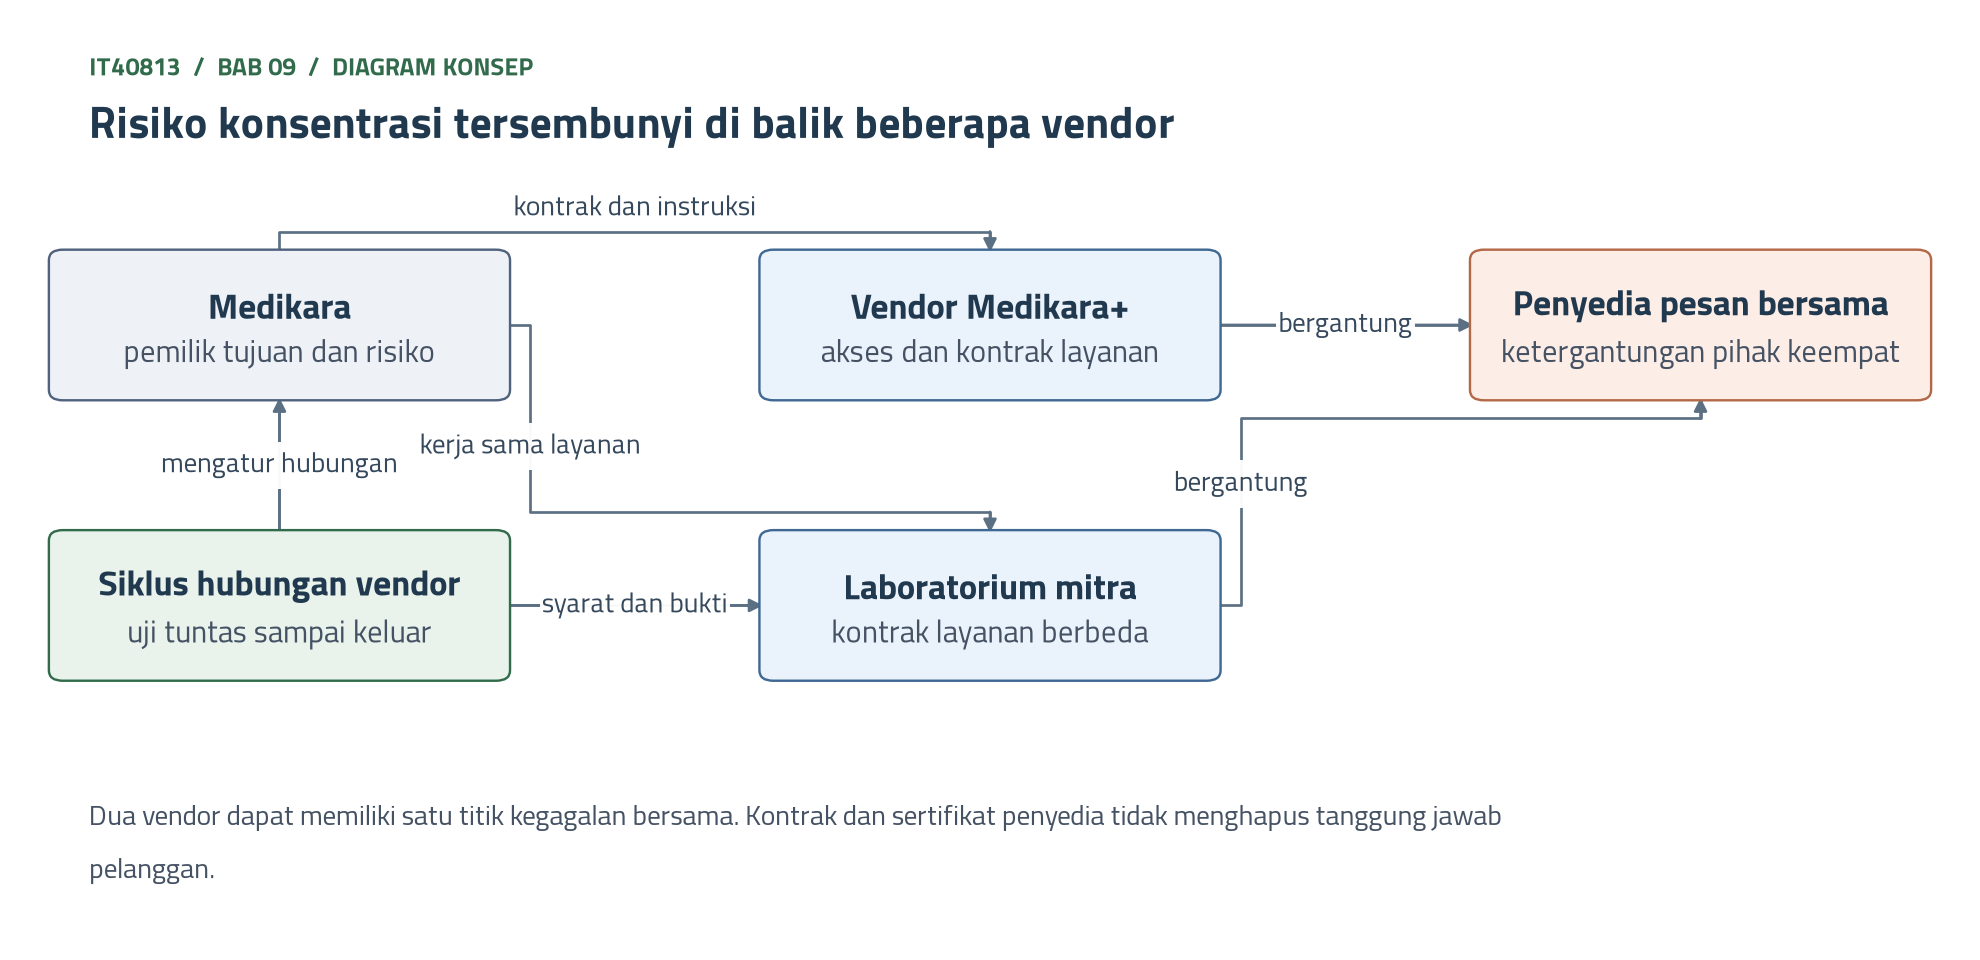
\includegraphics[width=0.96\textwidth,height=0.77\textheight,keepaspectratio]{../../figures/ch09-diagram-konsep.png}
  \label{fig:session09-ilustrasi-bab}
\end{frame}

\section{Rantai Pasok dan Konsentrasi}

\begin{frame}{{\Large Pihak Ketiga dan Pihak Keempat}}
  \vspace{6pt}
  \small
  \begin{itemize}
    \item Pihak ketiga: vendor aplikasi, penyedia cloud, mitra data, dan layanan pendukung.
    \item Pihak keempat: pemasok yang dipakai pihak ketiga.
    \item NIST CSF 2.0 menyebut ekosistem pasok dengan beberapa lapis alih daya.
    \item Analogi kantin: dua pedagang dari satu gudang tidak memberi keragaman pasokan.
    \item Jumlah kontrak tidak sama dengan jumlah sumber daya yang independen.
  \end{itemize}
\end{frame}

\begin{frame}{{\Large Menghitung Konsentrasi (Misalkan)}}
  \vspace{4pt}
  \small
  \begin{tabularx}{\textwidth}{|>{\raggedright\arraybackslash}X|>{\raggedright\arraybackslash}p{0.34\textwidth}|>{\raggedright\arraybackslash}p{0.24\textwidth}|}
    \hline
    \textbf{Keadaan} & \textbf{Hitungan} & \textbf{Gangguan bersamaan} \\ \hline
    Dua penyedia terpisah & 0,5\% kali 0,5\% kali 8.760 jam & Sekitar 13 menit per tahun \\ \hline
    Satu penyedia pesan & 0,5\% kali 8.760 jam & 43,8 jam per tahun \\ \hline
  \end{tabularx}

  \vspace{8pt}
  \begin{itemize}
    \item Selisihnya 200 kali lipat. Register Bab 5 mencatatnya sebagai R-08, skor $2 \times 4 = 8$.
    \item Pengingat 336.000 janji temu ikut terganggu sekitar 0,5 persen, atau 1.680 janji temu.
    \item 144 uji pemulihan dapat lulus tanpa menjawab cadangan di akun yang sama.
  \end{itemize}
\end{frame}

\begin{frame}{{\Large Peta Ketergantungan (Misalkan)}}
  \vspace{2pt}
  \begin{center}
    \resizebox{0.76\textwidth}{!}{\begin{tikzpicture}[
  font=\scriptsize,
  execute at begin node={\hyphenpenalty=10000},
  induk/.style={draw, rounded corners, align=center, text width=1.8cm,
    minimum height=1.3cm, fill=praditagreen!15},
  tahap/.style={draw, rounded corners, align=center, text width=3.1cm,
    minimum height=0.62cm, fill=blue!8},
  lanjut/.style={draw, rounded corners, align=center, text width=3.4cm,
    minimum height=0.62cm, fill=orange!12},
  masalah/.style={draw, rounded corners, align=center, text width=3.4cm,
    minimum height=0.9cm, fill=red!22},
  panah/.style={-{Stealth[length=2mm]}, thick}]
  \node[font=\scriptsize\bfseries] at (0,2.75) {Organisasi};
  \node[font=\scriptsize\bfseries] at (3.6,2.75) {Pihak ketiga};
  \node[font=\scriptsize\bfseries] at (8.1,2.75) {Pihak keempat};
  \node[induk] (m) at (0,0)
    {Medikara\\{\tiny\mdseries pemilik tujuan dan risiko}};
  \node[tahap] (v3) at (3.6,2) {V-03 Laboratorium mitra};
  \node[tahap] (v1) at (3.6,1) {V-01 Vendor Medikara+};
  \node[tahap] (v2) at (3.6,0) {V-02 Penyedia cloud};
  \node[tahap] (v4) at (3.6,-1) {V-04 Mitra asuransi};
  \node[tahap] (v5) at (3.6,-2) {V-05 Apotek daring};
  \node[masalah] (p1) at (8.1,1.6)
    {Penyedia pesan bersama\\{\tiny\mdseries titik kegagalan V-01 dan V-03}};
  \node[masalah] (p2) at (8.1,0.3)
    {Layanan identitas bersama\\{\tiny\mdseries titik kegagalan V-01 dan V-02}};
  \node[lanjut] (p3) at (8.1,-1) {Pengolah klaim};
  \node[lanjut] (p4) at (8.1,-2) {Kurir obat};
  \draw[panah] (m.east) -- (v3.west);
  \draw[panah] (m.east) -- (v1.west);
  \draw[panah] (m.east) -- (v2.west);
  \draw[panah] (m.east) -- (v4.west);
  \draw[panah] (m.east) -- (v5.west);
  \draw[panah] (v1.south) -- (v2.north);
  \draw[panah] (v3.east) -- (p1.west);
  \draw[panah] (v1.east) -- (p1.west);
  \draw[panah] (v1.east) -- (p2.west);
  \draw[panah] (v2.east) -- (p2.west);
  \draw[panah] (v4.east) -- (p3.west);
  \draw[panah] (v5.east) -- (p4.west);
\end{tikzpicture}
}
  \end{center}
  \footnotesize V-01 memakai 3 penyedia pendukung, sehingga Medikara perlu 3 persetujuan tertulis
  (Pasal 51 ayat (5) UU PDP).
\end{frame}

\begin{frame}{{\Large Membaca Tiga Sumber}}
  \vspace{2pt}
  \scriptsize
  \begin{tabularx}{\textwidth}{|>{\raggedright\arraybackslash}p{0.2\textwidth}|>{\raggedright\arraybackslash}X|>{\raggedright\arraybackslash}X|}
    \hline
    \textbf{Sumber} & \textbf{Angka} & \textbf{Batas pembacaan} \\ \hline
    Survei AHA, Change Healthcare & Hampir 1.000 rumah sakit: 94\% dampak keuangan, 83\% arus kas,
    74\% pelayanan langsung & Laporan mandiri, dibuat asosiasi rumah sakit \\ \hline
    NHS England London, Synnovis & Janji rawat jalan dan tindakan elektif ditunda pada dua
    \textit{trust}; angka rinci tidak dikutip & Data manajemen yang belum diverifikasi \\ \hline
    DBIR 2026 lewat WaterISAC & Pihak ketiga terlibat pada 48\% pelanggaran & Bagian dari
    pelanggaran, bukan peluang \\ \hline
  \end{tabularx}

  \vspace{8pt}
  \small Angka global tidak disalin menjadi peluang Medikara. Bab 5 tetap memakai peluang R-01
  sebesar 0,2 per tahun.
\end{frame}

\section{Siklus Hidup}

\begin{frame}{{\Large Siklus Kendali Pihak Ketiga}}
  \vspace{6pt}
  \begin{center}
    \resizebox{0.96\textwidth}{!}{\begin{tikzpicture}[
  font=\scriptsize,
  execute at begin node={\hyphenpenalty=10000},
  tahap/.style={draw, rounded corners, align=center, text width=1.85cm,
    minimum height=1.2cm, fill=blue!8},
  catatan/.style={align=center, font=\tiny\mdseries},
  panah/.style={-{Stealth[length=2mm]}, thick}]
  \node[tahap] (n0) at (0,0) {Klasifikasi\\{\tiny\mdseries GV.SC-04}};
  \node[tahap] (n1) at (2.5,0) {Uji tuntas\\{\tiny\mdseries GV.SC-06}};
  \node[tahap, fill=orange!12] (n2) at (5,0) {Kontrak\\{\tiny\mdseries GV.SC-05}};
  \node[tahap] (n3) at (7.5,0) {Penerapan dan pemantauan\\{\tiny\mdseries GV.SC-07}};
  \node[tahap, fill=green!10] (n4) at (10,0) {Keluar dan verifikasi\\{\tiny\mdseries GV.SC-10}};
  \node[tahap, fill=red!22] (ins) at (7.5,-2) {Insiden bersama\\{\tiny\mdseries GV.SC-08}};
  \draw[panah] (n0) -- (n1);
  \draw[panah] (n1) -- (n2);
  \draw[panah] (n2) -- (n3);
  \draw[panah] (n3) -- (n4);
  \draw[panah] (n3) -- (ins);
  \draw[panah, rounded corners] (ins.west) -| (n2.south);
  \draw[panah, rounded corners] (n3.north) -- ++(0,0.45) -| (n0.north);
  \node[catatan] at (3.75,1.32)
    {perubahan tujuan, subprosesor, lokasi, atau skala memicu klasifikasi ulang};
  \node[catatan, anchor=east] at (6.3,-2.2) {temuan memperbaiki klausul};
\end{tikzpicture}
}
  \end{center}
  \small Analogi sewa kendaraan: periksa saat menerima, catat aturan, pantau gangguan, periksa saat
  mengembalikan.
\end{frame}

\begin{frame}{{\Large Tahap, Hasil, dan Bukti (Misalkan)}}
  \vspace{2pt}
  \scriptsize
  \begin{tabularx}{\textwidth}{|>{\raggedright\arraybackslash}p{0.25\textwidth}|>{\raggedright\arraybackslash}p{0.13\textwidth}|>{\raggedright\arraybackslash}X|}
    \hline
    \textbf{Tahap} & \textbf{Hasil} & \textbf{Bukti pada Medikara} \\ \hline
    Klasifikasi & GV.SC-04 & Register pemasok dengan skor \\ \hline
    Uji tuntas & GV.SC-06 & Kuesioner beserta bukti dan cakupan \\ \hline
    Kontrak & GV.SC-05 & 11 dari 11 butir; klausul K-05 \\ \hline
    Penerapan dan pemantauan & GV.SC-07 & 60 dari 60 catatan AC-01; tinjauan triwulanan \\ \hline
    Insiden bersama & GV.SC-08 & 2 latihan per tahun; laporan 12 jam \\ \hline
    Keluar & GV.SC-10 & Hasil uji ekspor dan bukti penghapusan \\ \hline
  \end{tabularx}

  \vspace{8pt}
  \small Hanya GV.SC-07 yang masuk profil target Bab 8. Lima baris lain menjadi pertanyaan kerja.
\end{frame}

\begin{frame}{{\Large Klasifikasi Enam Hubungan (Misalkan)}}
  \vspace{2pt}
  \scriptsize
  \begin{tabularx}{\textwidth}{|>{\raggedright\arraybackslash}p{0.08\textwidth}|>{\raggedright\arraybackslash}X|*{4}{>{\centering\arraybackslash}p{0.08\textwidth}|}>{\raggedright\arraybackslash}p{0.16\textwidth}|}
    \hline
    \textbf{ID} & \textbf{Hubungan} & \textbf{Data} & \textbf{Kritis} & \textbf{Ganti} &
    \textbf{Skor} & \textbf{Tingkat} \\ \hline
    V-01 & Vendor Medikara+ & 3 & 3 & 3 & 9 & Terperinci \\ \hline
    V-02 & Penyedia cloud & 3 & 3 & 2 & 8 & Terperinci \\ \hline
    V-03 & Laboratorium mitra & 3 & 3 & 2 & 8 & Terperinci \\ \hline
    V-04 & Mitra asuransi & 3 & 2 & 2 & 7 & Terperinci \\ \hline
    V-05 & Apotek daring & 2 & 2 & 1 & 5 & Menengah \\ \hline
    V-06 & Penyedia cetak materi & 0 & 0 & 1 & 1 & Dasar \\ \hline
  \end{tabularx}

  \vspace{8pt}
  \small Skor 7 sampai 9 terperinci, 4 sampai 6 menengah, 0 sampai 3 dasar. Skala ini rancangan
  pembelajaran, bukan rumus standar.
\end{frame}

\begin{frame}{{\Large Mengapa Pemeriksaan Dibuat Bertingkat}}
  \vspace{6pt}
  \small
  \begin{itemize}
    \item Analogi tamu rumah sakit: pengantar bunga mendaftar di lobi, teknisi ruang obat perlu
          surat tugas dan pendamping.
    \item Misalkan 40 hubungan: 5 terperinci, 12 menengah, 23 dasar.
    \item Pada 40, 16, dan 4 jam per hubungan, totalnya 484 jam, atau Rp29,04 juta.
    \item Bila semua diperiksa terperinci: 1.600 jam, atau Rp96 juta.
    \item Pembagian tingkat menghemat 1.116 jam, sekitar 70 persen.
  \end{itemize}
\end{frame}

\begin{frame}{{\Large Uji Tuntas: Dari Jawaban ke Bukti}}
  \vspace{2pt}
  \scriptsize
  \begin{tabularx}{\textwidth}{|>{\raggedright\arraybackslash}p{0.26\textwidth}|>{\raggedright\arraybackslash}X|>{\raggedright\arraybackslash}X|}
    \hline
    \textbf{Jenis bukti} & \textbf{Contoh} & \textbf{Yang diperiksa} \\ \hline
    1. Jawaban vendor & Kuesioner, CAIQ & Tanggal dan siapa yang menjawab \\ \hline
    2. Dokumen vendor & Kebijakan, prosedur & Apakah dijalankan pada layanan itu \\ \hline
    3. Laporan independen & Sertifikat, laporan SOC 2 & Cakupan, periode, pengecualian \\ \hline
    4. Uji bersama & Uji ekspor, latihan insiden & Hasil, kekurangan, uji ulang \\ \hline
  \end{tabularx}

  \vspace{8pt}
  \small
  \begin{itemize}
    \item Misalkan 10 dari 10 jawaban ya, tetapi hanya 7 punya bukti dalam cakupan: 70 persen.
    \item Skor eksternal dari informasi publik tidak sepenuhnya menyatu (Keskin dan rekan, 2021).
  \end{itemize}
\end{frame}

\begin{frame}{{\Large Pemantauan Sepanjang Hubungan (Misalkan)}}
  \vspace{2pt}
  \scriptsize
  \begin{tabularx}{\textwidth}{|>{\raggedright\arraybackslash}X|>{\raggedright\arraybackslash}p{0.22\textwidth}|>{\raggedright\arraybackslash}X|}
    \hline
    \textbf{Indikator} & \textbf{Ambang} & \textbf{Tindakan bila terlewati} \\ \hline
    Akun vendor tanpa pemilik & 0 akun (Bab 5) & Bekukan akun dan catat penyimpangan \\ \hline
    Catatan peninjauan AC-01 & 60 dari 60 per tahun & Eskalasi ke kepala TI \\ \hline
    Laporan dugaan insiden & 12 jam (K-05) & Catat pelanggaran dan tagih perbaikan \\ \hline
    Latihan insiden bersama & 2 per tahun & Masuk temuan Paket C \\ \hline
    Pemberitahuan subprosesor & 30 hari sebelumnya & Tunda perubahan atau putuskan risiko sisa \\
    \hline
    Uji ekspor & 1 per tahun & Tinjau ulang skor R-10 \\ \hline
  \end{tabularx}

  \vspace{6pt}
  \small Tinjauan paralel Bab 8 memakan 10 hari kerja, sekitar 14 hari kalender. Dari 30 hari,
  tersisa 16 hari untuk menguji layanan pengganti.
\end{frame}

\begin{frame}{{\Large Strategi Keluar Perlu Diuji}}
  \vspace{2pt}
  \scriptsize
  \begin{tabularx}{\textwidth}{|>{\raggedright\arraybackslash}X|>{\raggedright\arraybackslash}p{0.13\textwidth}|>{\raggedright\arraybackslash}p{0.2\textwidth}|>{\raggedright\arraybackslash}p{0.13\textwidth}|>{\raggedright\arraybackslash}p{0.11\textwidth}|}
    \hline
    \textbf{Opsi R-10} & \textbf{Biaya sekali} & \textbf{Harapan setelahnya} &
    \textbf{Turun per tahun} & \textbf{Balik modal} \\ \hline
    Uji ekspor dan pendampingan & Rp60 juta & 0,1 kali Rp300 juta, atau Rp30 juta & Rp50 juta & 1,2
    tahun \\ \hline
    Ganti vendor segera & Rp300 juta & 0,05 kali Rp800 juta, atau Rp40 juta & Rp40 juta & 7,5 tahun
    \\ \hline
  \end{tabularx}

  \vspace{8pt}
  \small
  \begin{itemize}
    \item Awal: peluang 0,1 dan kerugian Rp800 juta, harapan Rp80 juta per tahun.
    \item Uji 10.000 rekam sintetis: 96 persen terbaca mesin. Sisa 13.440 rekam per tahun memakan
          1.120 jam, atau Rp67,2 juta.
    \item Vendor baru dapat memakai subpenyedia yang sama, sehingga R-08 tidak berubah.
  \end{itemize}
\end{frame}

\begin{frame}{{\Large Kasus Medikara: Dua Prioritas}}
  \vspace{6pt}
  \small
  \begin{itemize}
    \item Empat dari lima hubungan target masuk tingkat terperinci.
    \item V-01 terpilih dengan skor 9. V-02 dan V-03 sama-sama 8.
    \item Pemutus tambahan: jumlah layanan yang berhenti. V-02 menampung seluruh platform target.
    \item Bab 8 menganggarkan Rp120 juta per tahun untuk APO10 tingkat 3, sedangkan R-10 turun Rp50
          juta.
    \item Selisihnya dibenarkan oleh K-05 yang tidak memenuhi dan oleh hak pasien.
  \end{itemize}
\end{frame}

\section{Klausul Kontrak}

\begin{frame}{{\Large Dari Janji Menjadi Ukuran}}
  \vspace{6pt}
  \small
  \begin{itemize}
    \item Kontrak menerjemahkan kendali menjadi kewajiban yang dapat ditagih.
    \item Analogi pengiriman: ``barang dijaga'' belum menjelaskan siapa menerima dan kapan
          terlambat.
    \item ``Secepatnya'' tidak dapat ditagih. K-05 menetapkan 12 jam sejak vendor mendeteksi.
    \item ``Menjaga kerahasiaan'' tidak menjawab akun yang tetap aktif. Akun dicabut dalam 1 hari
          kerja.
    \item Angka 12 jam pilihan kontrak, bukan tenggat undang-undang.
  \end{itemize}
\end{frame}

\begin{frame}{{\Large Klausul 12 Jam pada Garis Waktu (Misalkan)}}
  \vspace{6pt}
  \begin{center}
    \resizebox{0.92\textwidth}{!}{\begin{tikzpicture}[
  font=\scriptsize,
  execute at begin node={\hyphenpenalty=10000},
  atas/.style={align=center, text width=1.6cm, inner sep=0pt, anchor=south},
  bawah/.style={align=center, text width=1.6cm, inner sep=0pt, anchor=north,
    font=\tiny\mdseries},
  rentang/.style={{Stealth[length=1.6mm]}-{Stealth[length=1.6mm]}, thick},
  nilai/.style={fill=white, inner sep=1pt, font=\tiny\bfseries}]
  \fill[green!10] (0,0) rectangle (1.68,0.28);
  \fill[red!22] (1.68,0) rectangle (4.2,0.28);
  \fill[blue!8] (4.2,0) rectangle (8.4,0.28);
  \fill[orange!12] (8.4,0) rectangle (10.08,0.28);
  \draw (0,0) rectangle (10.08,0.28);
  \foreach \x in {0,1.68,4.2,8.4,10.08} {
    \draw[thick] (\x,-0.08) -- (\x,0.36);
  }
  \node[atas] at (0,0.42) {Jam 0\\{\tiny\mdseries Jumat 20.00}};
  \node[atas] at (1.68,0.42) {Jam 12\\{\tiny\mdseries Sabtu 08.00}};
  \node[atas] at (4.2,0.42) {Jam 30\\{\tiny\mdseries Minggu 02.00}};
  \node[atas] at (8.4,0.42) {Jam 60\\{\tiny\mdseries Senin 08.00}};
  \node[atas] at (10.08,0.42) {Jam 72\\{\tiny\mdseries Senin 20.00}};
  \node[bawah] at (0,-0.14) {Vendor mendeteksi};
  \node[bawah] at (1.68,-0.14) {Batas K-05};
  \node[bawah] at (4.2,-0.14) {Varian Bab 3: terlambat 18 jam};
  \node[bawah] at (8.4,-0.14) {Batas internal naskah};
  \node[bawah] at (10.08,-0.14) {Batas terluar Pasal 46};
  \draw[rentang] (1.68,-1.02) -- node[nilai] {48 jam} (8.4,-1.02);
  \draw[rentang] (1.68,-1.42) -- node[nilai] {60 jam} (10.08,-1.42);
  \draw[rentang] (4.2,-1.82) -- node[nilai] {30 jam} (8.4,-1.82);
  \draw[rentang] (4.2,-2.22) -- node[nilai] {42 jam} (10.08,-2.22);
  \node[align=right, anchor=east, font=\tiny\mdseries] at (1.6,-1.22)
    {laporan pada\\jam ke-12};
  \node[align=right, anchor=east, font=\tiny\mdseries] at (4.12,-2.02)
    {laporan pada\\jam ke-30};
\end{tikzpicture}
}
  \end{center}
  \footnotesize Mengandaikan kegagalan dan penemuan bersamaan. Pasal 46 ayat (1) tidak memakai frasa
  sejak diketahui secara eksplisit, sehingga fungsi hukum menetapkan titik mulainya.
\end{frame}

\begin{frame}{{\Large Sembilan Pokok Klausul: Akses dan Insiden}}
  \vspace{2pt}
  \scriptsize
  \begin{tabularx}{\textwidth}{|>{\raggedright\arraybackslash}p{0.26\textwidth}|>{\raggedright\arraybackslash}X|>{\raggedright\arraybackslash}X|}
    \hline
    \textbf{Pokok} & \textbf{Ukuran penerimaan} & \textbf{Bukti} \\ \hline
    Instruksi dan batas tujuan & Tujuan tertulis; perubahan lewat persetujuan & Daftar instruksi
    berversi \\ \hline
    Pengguna dan peninjauan akses & Pemilik dan tanggal berakhir; cabut dalam 1 hari kerja & 120
    dari 120 akun cocok; AC-01 \\ \hline
    Subprosesor & Persetujuan tertulis; pemberitahuan 30 hari & Daftar penerima dan persetujuan \\
    \hline
    Lokasi dan akses dukungan & Di dalam wilayah Indonesia, kecuali izin sesuai Pasal 972 &
    Inventaris lokasi data, cadangan, dan akses \\ \hline
    Laporan dugaan insiden & Laporan awal 12 jam; 2 latihan per tahun & Kronologi dan hasil latihan
    \\ \hline
  \end{tabularx}
\end{frame}

\begin{frame}{{\Large Sembilan Pokok Klausul: Bukti dan Keluar}}
  \vspace{2pt}
  \scriptsize
  \begin{tabularx}{\textwidth}{|>{\raggedright\arraybackslash}p{0.26\textwidth}|>{\raggedright\arraybackslash}X|>{\raggedright\arraybackslash}X|}
    \hline
    \textbf{Pokok} & \textbf{Ukuran penerimaan} & \textbf{Bukti} \\ \hline
    Catatan aktivitas & Per orang; disimpan 90 hari & Uji telusur satu rekam \\ \hline
    Pemeriksaan dan asurans & Bukti dapat ditinjau sesuai cakupan & Laporan, pengecualian, dan
    tindak lanjut \\ \hline
    Ekspor dan biaya keluar & Format dan tenggat disepakati; ekspor lengkap & Hasil uji ekspor
    tahunan \\ \hline
    Penghapusan dan cadangan & Terverifikasi, termasuk salinan cadangan & Berita acara penghapusan
    \\ \hline
  \end{tabularx}

  \vspace{8pt}
  \small Ganti rugi dapat memindahkan biaya Rp23,7 juta. Kewajiban Pasal 46 tetap pada Medikara, dan
  kepercayaan pasien tidak berpindah lewat kontrak.
\end{frame}

\begin{frame}{{\Large Enam dari Sebelas Butir}}
  \vspace{6pt}
  \small
  \begin{itemize}
    \item Salinan pihak ketiga PP 33/2026 Pasal 14 memuat 11 butir. Naskah resmi belum diperoleh,
          jadi dipakai sebagai daftar periksa.
    \item Bab 7: perjanjian memuat 6 dari 11 butir. Bab 8 menargetkan 11 dari 11.
    \item Lima pokok tawar ulang (penafsiran bab): instruksi, daftar akun dan subprosesor,
          pencabutan akses, pengawasan dan audit, pengembalian dan penghapusan.
    \item Laporan 12 jam sudah ada pada K-05: jawabannya latihan. Waktu pulih kontrak (V-01 24 jam,
          layanan identitas 8 jam) ditawar tersendiri pada Bab 10.
    \item K-12 berjalan sebaliknya: Medikara melapor ke mitra asuransi dalam 1 jam, 2 dari 12 tepat
          waktu.
  \end{itemize}
\end{frame}

\begin{frame}{{\Large Kasus Medikara: Klausul untuk Insiden 2025}}
  \vspace{2pt}
  \scriptsize
  \begin{tabularx}{\textwidth}{|>{\raggedright\arraybackslash}p{0.24\textwidth}|>{\raggedright\arraybackslash}p{0.24\textwidth}|>{\raggedright\arraybackslash}X|}
    \hline
    \textbf{Klausul} & \textbf{Ukuran} & \textbf{Akibat pada kronologi} \\ \hline
    Pencabutan akun & 1 hari kerja setelah penugasan selesai & Akun tidak aktif pada malam pertama
    \\ \hline
    Pemantauan dan laporan & Laporan dugaan insiden 12 jam & Deteksi malam pertama: 155 rekam, turun
    87,5 persen. Setelah dua malam: 310, turun 75 persen \\ \hline
    Catatan aktivitas & Per orang; 90 hari & Seluruh 8 malam tertelusur, bukan hanya 620 rekam \\
    \hline
  \end{tabularx}

  \vspace{8pt}
  \small Klausul tidak menjawab bahwa Medikara tahu lewat keluhan pasien. Tinjauan catatan aktivitas
  di sisi Medikara masuk Paket D.
\end{frame}

\section{Cloud}

\begin{frame}{{\Large Tanggung Jawab Bersama}}
  \vspace{6pt}
  \small
  \begin{itemize}
    \item NIST SP 800-145: lima karakteristik, tiga model layanan, empat model penyebaran.
    \item IaaS, PaaS, dan SaaS memindahkan lapisan operasi yang berbeda.
    \item AWS: \textit{security of the cloud} milik penyedia, \textit{security in the cloud} milik
          pelanggan.
    \item Analogi sewa tempat: pengelola menjaga gedung, penyewa mengatur kunci dan dokumen.
    \item Pasal 51 ayat (3) UU PDP: pemrosesan oleh prosesor termasuk tanggung jawab pengendali.
  \end{itemize}
\end{frame}

\begin{frame}{{\Large Pembagian Lapisan Menurut Panduan Microsoft}}
  \vspace{2pt}
  \begin{center}
    \resizebox{0.72\textwidth}{!}{\begin{tikzpicture}[
  font=\scriptsize,
  lapisan/.style={draw, align=left, text width=3.5cm, minimum height=0.42cm, inner xsep=3pt,
    inner ysep=0pt, fill=praditagreen!15},
  judul/.style={draw, align=center, minimum width=2.3cm, minimum height=0.42cm,
    inner ysep=0pt, fill=praditagreen!15, font=\scriptsize\bfseries},
  pel/.style={draw, align=center, minimum width=2.3cm, minimum height=0.42cm, inner ysep=0pt,
    fill=orange!12},
  ber/.style={draw, align=center, minimum width=2.3cm, minimum height=0.42cm, inner ysep=0pt,
    fill=blue!8},
  pen/.style={draw, align=center, minimum width=2.3cm, minimum height=0.42cm, inner ysep=0pt,
    fill=green!10}]
  \node[lapisan, font=\scriptsize\bfseries] at (0,0) {Lapisan};
  \node[judul] at (3.2,0) {IaaS};
  \node[judul] at (5.5,0) {PaaS};
  \node[judul] at (7.8,0) {SaaS};
  \node[lapisan] at (0,-0.42) {Data pelanggan};
  \node[pel] at (3.2,-0.42) {Pelanggan};
  \node[pel] at (5.5,-0.42) {Pelanggan};
  \node[pel] at (7.8,-0.42) {Pelanggan};
  \node[lapisan] at (0,-0.84) {Konfigurasi dan pengaturan};
  \node[pel] at (3.2,-0.84) {Pelanggan};
  \node[pel] at (5.5,-0.84) {Pelanggan};
  \node[pel] at (7.8,-0.84) {Pelanggan};
  \node[lapisan] at (0,-1.26) {Identitas dan pengguna};
  \node[pel] at (3.2,-1.26) {Pelanggan};
  \node[pel] at (5.5,-1.26) {Pelanggan};
  \node[pel] at (7.8,-1.26) {Pelanggan};
  \node[lapisan] at (0,-1.68) {Perangkat klien};
  \node[pel] at (3.2,-1.68) {Pelanggan};
  \node[pel] at (5.5,-1.68) {Pelanggan};
  \node[ber] at (7.8,-1.68) {Bersama};
  \node[lapisan] at (0,-2.1) {Aplikasi};
  \node[pel] at (3.2,-2.1) {Pelanggan};
  \node[ber] at (5.5,-2.1) {Bersama};
  \node[ber] at (7.8,-2.1) {Bersama};
  \node[lapisan] at (0,-2.52) {Kendali jaringan};
  \node[pel] at (3.2,-2.52) {Pelanggan};
  \node[ber] at (5.5,-2.52) {Bersama};
  \node[pen] at (7.8,-2.52) {Penyedia};
  \node[lapisan] at (0,-2.94) {Sistem operasi};
  \node[pel] at (3.2,-2.94) {Pelanggan};
  \node[pen] at (5.5,-2.94) {Penyedia};
  \node[pen] at (7.8,-2.94) {Penyedia};
  \node[lapisan] at (0,-3.36) {Host fisik};
  \node[pen] at (3.2,-3.36) {Penyedia};
  \node[pen] at (5.5,-3.36) {Penyedia};
  \node[pen] at (7.8,-3.36) {Penyedia};
  \node[lapisan] at (0,-3.78) {Jaringan fisik};
  \node[pen] at (3.2,-3.78) {Penyedia};
  \node[pen] at (5.5,-3.78) {Penyedia};
  \node[pen] at (7.8,-3.78) {Penyedia};
  \node[lapisan] at (0,-4.2) {Pusat data fisik};
  \node[pen] at (3.2,-4.2) {Penyedia};
  \node[pen] at (5.5,-4.2) {Penyedia};
  \node[pen] at (7.8,-4.2) {Penyedia};
\end{tikzpicture}
}
  \end{center}
  \footnotesize Panduan itu ilustratif dan tidak mengubah perjanjian. Pelanggan memegang penuh 7, 4,
  dan 3 dari 10 lapisan. Pada SaaS, 5 dari 10 lapisan masih memerlukan kerja pelanggan.
\end{frame}

\begin{frame}{{\Large Dua Contoh: Pekerjaan Tidak Hilang}}
  \vspace{6pt}
  \small
  \begin{itemize}
    \item Misalkan IaaS untuk 40 server virtual, pembaruan 1 jam per server per bulan.
    \item Bebannya 480 jam per tahun, atau Rp28,8 juta, sekitar 4,2 persen kapasitas tim platform 6
          orang.
    \item Misalkan SaaS: penyedia mengoperasikan aplikasi, Medikara tetap mengatur pengguna.
    \item Peninjauan 120 akun menghasilkan 60 catatan per tahun, dan itu pekerjaan Medikara.
    \item Isi matriks dari rancangan IT40713, bukan dari nama model saja.
  \end{itemize}
\end{frame}

\begin{frame}{{\Large Empat Bentuk Bukti Penyedia}}
  \vspace{2pt}
  \scriptsize
  \begin{tabularx}{\textwidth}{|>{\raggedright\arraybackslash}p{0.24\textwidth}|>{\raggedright\arraybackslash}X|>{\raggedright\arraybackslash}X|}
    \hline
    \textbf{Bentuk} & \textbf{Yang dijawab} & \textbf{Yang harus dibaca} \\ \hline
    CAIQ & Apa yang dinyatakan penyedia & Versi, tanggal, layanan, dan bukti tiap jawaban ya \\
    \hline
    Sertifikat ISO/IEC 27001 & Apakah sistem manajemen memenuhi persyaratan pada ruang lingkup itu &
    Ruang lingkup, lokasi, masa berlaku, dan penerbit \\ \hline
    SOC 2 Type 1 & Apakah kendali dirancang dan diterapkan pada satu tanggal & Tanggal, kategori,
    dan uraian sistem \\ \hline
    SOC 2 Type 2 & Apakah kendali bekerja selama satu periode & Periode, pengecualian, kontrol
    pelengkap \\ \hline
  \end{tabularx}

  \vspace{8pt}
  \small CCM versi 4.1 memuat 197 objektif kontrol dalam 17 domain. Jawaban ya tetap klaim yang
  perlu dibuktikan.
\end{frame}

\begin{frame}{{\Large Membaca Bukti: Dua Contoh}}
  \vspace{6pt}
  \small
  \begin{itemize}
    \item Sertifikat vendor berlaku 14 bulan, tetapi cakupannya hanya pengembangan aplikasi. Akun
          dukungan tidak termasuk.
    \item Laporan SOC 2 Type 2 mencakup Januari sampai Juni 2026. Dibaca 1 November, empat bulan
          belum tercakup.
    \item Pengujian mencatat 3 pengecualian dari 25 sampel pencabutan akses: 12 persen.
    \item Dari 14 kontrol pelengkap pengguna, Medikara baru menjalankan 9.
    \item Lima sisanya pekerjaan Medikara, bukan pekerjaan penyedia.
  \end{itemize}
\end{frame}

\begin{frame}{{\Large Lokasi Data dan Akses Dukungan}}
  \vspace{2pt}
  \scriptsize
  \begin{tabularx}{\textwidth}{|>{\raggedright\arraybackslash}p{0.2\textwidth}|>{\raggedright\arraybackslash}X|>{\raggedright\arraybackslash}X|}
    \hline
    \textbf{Aspek} & \textbf{Pertanyaan} & \textbf{Dasar penelusuran} \\ \hline
    Pusat data & Di mana data aktif disimpan? & PP 28/2024 Pasal 966 ayat (2) \\ \hline
    Cadangan & Di mana salinan cadangan berada? & Pasal 966; Permenkes 24/2022 Pasal 20 \\ \hline
    Jasa pihak lain & Apakah data tetap dikendalikan penuh? & Pasal 966 ayat (5); Permenkes Pasal 22
    \\ \hline
    Akses dukungan & Dari negara mana staf dapat melihat data? & Pasal 971 ayat (2) dan Pasal 972 \\
    \hline
    Transfer & Apakah ada tujuan spesifik dan izin? & Pasal 972; UU PDP Pasal 56 \\ \hline
  \end{tabularx}

  \vspace{6pt}
  \small
  \begin{itemize}
    \item Tawaran Rp420 juta, hemat Rp180 juta, berhenti pada Pasal 966 ayat (2).
    \item 4 staf luar negeri, 300 tiket per bulan: dukungan dalam negeri Rp300 juta per tahun lebih
          mahal.
  \end{itemize}
\end{frame}

\section{Berbagi Data dan DPIA}

\begin{frame}{{\Large DPIA Berfokus pada Dampak Pasien}}
  \vspace{6pt}
  \small
  \begin{itemize}
    \item Pasal 34 UU PDP: DPIA wajib bila pemrosesan berpotensi risiko tinggi.
    \item Alur klaim 72.000 per tahun menyentuh data spesifik, skala besar, dan penggabungan data.
    \item Analogi jalan perumahan: jalan baru mengubah keselamatan penghuni, bukan hanya pendapatan.
    \item Misalkan asuransi meminta riwayat 10.000 pasien untuk kepesertaan.
    \item Nilai apakah status minimum memenuhi tujuan tanpa riwayat lengkap.
  \end{itemize}
\end{frame}

\begin{frame}{{\Large Alur DPIA (Penafsiran Bab)}}
  \vspace{2pt}
  \begin{center}
    \resizebox{0.88\textwidth}{!}{\begin{tikzpicture}[
  font=\scriptsize,
  execute at begin node={\hyphenpenalty=10000},
  tahap/.style={draw, rounded corners, align=center, text width=2.35cm,
    minimum height=1.05cm, fill=blue!8},
  panah/.style={-{Stealth[length=2mm]}, thick}]
  \node[tahap] (n1) at (0,0)
    {Pemicu Pasal 34\\{\tiny\mdseries tujuh keadaan ayat (2)}};
  \node[tahap] (n2) at (3,0)
    {Tujuan dan kebutuhan\\{\tiny\mdseries data apa yang perlu}};
  \node[tahap] (n3) at (6,0)
    {Peta data\\{\tiny\mdseries sumber, penerima, lokasi}};
  \node[tahap] (n4) at (9,0)
    {Dampak pada pasien\\{\tiny\mdseries bukan hanya rupiah}};
  \node[tahap] (n5) at (9,-1.75)
    {Kontrol dan risiko sisa\\{\tiny\mdseries bukti uji sebelum aktif}};
  \node[tahap, fill=orange!12] (n6) at (6,-1.75)
    {Keputusan tujuan\\{\tiny\mdseries direktur pelayanan}};
  \node[tahap, fill=green!10] (n7) at (3,-1.75)
    {Aktif dengan syarat\\{\tiny\mdseries pemilik layanan}};
  \node[tahap] (n8) at (0,-1.75)
    {Pantau dan tinjau ulang\\{\tiny\mdseries bila tujuan atau skala berubah}};
  \node[tahap, fill=red!22] (n9) at (6,-3.5)
    {Hentikan atau naik\\{\tiny\mdseries risiko sisa di atas batas ke direksi}};
  \draw[panah] (n1) -- (n2);
  \draw[panah] (n2) -- (n3);
  \draw[panah] (n3) -- (n4);
  \draw[panah] (n4) -- (n5);
  \draw[panah] (n5) -- (n6);
  \draw[panah] (n6) -- (n7);
  \draw[panah] (n7) -- (n8);
  \draw[panah] (n6) -- node[right, align=left, font=\tiny\mdseries]
    {kurangi data,\\nilai ulang} (n3);
  \draw[panah] (n6) -- (n9);
\end{tikzpicture}
}
  \end{center}
\end{frame}

\begin{frame}{{\Large Mengurangi Data Lebih Dahulu (Misalkan)}}
  \vspace{2pt}
  \scriptsize
  \begin{tabularx}{\textwidth}{|>{\raggedright\arraybackslash}X|>{\raggedright\arraybackslash}p{0.3\textwidth}|>{\centering\arraybackslash}p{0.1\textwidth}|>{\raggedright\arraybackslash}p{0.17\textwidth}|}
    \hline
    \textbf{Pilihan} & \textbf{Rekam} & \textbf{Kolom} & \textbf{Nilai data} \\ \hline
    Riwayat lengkap & $10.000 \times 30 = 300.000$ & 42 & 12.600.000 \\ \hline
    Klaim lengkap & 72.000 per tahun & 42 & 3.024.000 \\ \hline
    Data minimum & 72.000 per tahun & 9 & 648.000 \\ \hline
  \end{tabularx}

  \vspace{8pt}
  \small
  \begin{itemize}
    \item Data minimum turun sekitar 94,9 persen dari riwayat lengkap, dan 78,6 persen dari klaim
          lengkap.
    \item Nilai data adalah ukuran paparan, bukan ukuran risiko.
    \item Enkripsi tidak menghapus risiko penggunaan berlebih oleh penerima sah.
  \end{itemize}
\end{frame}

\begin{frame}{{\Large Kasus Medikara: DPIA Alur Asuransi}}
  \vspace{6pt}
  \small
  \begin{itemize}
    \item CP-03: DPIA alur asuransi belum ada, dan Bab 8 menjadikannya syarat.
    \item DPIA dikerjakan 3 orang selama 3 hari, atau 72 jam, atau Rp4,32 juta.
    \item Mitra meminta 1 bulan untuk mengubah sistem. Klaim manual: 500 jam, atau Rp30 juta.
    \item Direktur pelayanan memutuskan menunggu, dan alasannya tercatat.
    \item Perubahan tujuan, kolom, penerima, lokasi, atau skala memicu penilaian ulang.
  \end{itemize}
\end{frame}

\section{Aktivitas, Ringkasan, dan Latihan}

\begin{frame}{{\Large Aktivitas: Kerangka Pihak Ketiga dan DPIA}}
  \vspace{6pt}
  \small
  \begin{itemize}
    \item Klasifikasi lima hubungan, dan peta pihak keempat yang dipakai lebih dari satu hubungan.
    \item Pilih dua hubungan kritis untuk uji tuntas, klausul, indikator, dan strategi keluar.
    \item Isi matriks layanan cloud dari rancangan IT40713.
    \item Susun DPIA satu alur asuransi.
    \item Simulasikan dugaan insiden Jumat 20.00, dengan laporan sebelum Sabtu 08.00.
  \end{itemize}
\end{frame}

\begin{frame}{{\Large Peran, Luaran C3, dan Berkas}}
  \vspace{6pt}
  \small
  \begin{itemize}
    \item Peran: bisnis menilai kekritisan, analis regulasi memimpin klausul dan DPIA, analis
          teknologi mengisi matriks, analis risiko menautkan R-01, R-08, dan R-10.
    \item Rubrik: klasifikasi dan bukti, kontrak dan pemantauan, kejelasan tanggung jawab, serta
          dampak dan risiko sisa, masing-masing 25 persen.
    \item Berkas ada di \berkas{sources/chapter09/}, dengan daftar pada \berkas{README.md}.
    \item Data pasien dan rahasia akses tidak boleh masuk folder tugas.
    \item Pendalaman opsional: CCM seri 4, SBOM, dan laporan uji penetrasi.
  \end{itemize}
\end{frame}

\begin{frame}{{\Large Ringkasan}}
  \vspace{6pt}
  \small
  \begin{itemize}
    \item Banyak vendor dapat memiliki satu titik kegagalan bersama.
    \item Uji tuntas hanya awal. Kontrak, pemantauan, perubahan, dan keluar butuh pemilik serta
          bukti.
    \item Klausul 12 jam memberi 48 jam sampai batas internal, tanpa memindahkan kewajiban Pasal 46.
    \item Cloud membagi pekerjaan: pada SaaS, 5 dari 10 lapisan masih memerlukan kerja pelanggan.
    \item DPIA menilai akibat pada pasien. Mengurangi data lebih dahulu, baru menambah kontrol.
  \end{itemize}
\end{frame}

\begin{frame}{{\Large Latihan}}
  \vspace{6pt}
  \small
  \begin{itemize}
    \item Latihan 1. Jelaskan mengapa sertifikat ISO/IEC 27001 milik penyedia cloud tidak
          memindahkan seluruh tanggung jawab keamanan kepada penyedia.
    \item Latihan 2. Susun tiga klausul kontrak yang dapat mencegah atau membatasi dampak insiden
          seperti kebocoran lewat vendor pada 2025.
    \item Latihan 3. Kapan alur berbagi data dengan mitra wajib didahului DPIA? Jelaskan dengan
          contoh.
  \end{itemize}
\end{frame}

\begin{frame}{{\Large Bacaan dan Pesan Utama}}
  \vspace{4pt}
  \small
  \href{https://doi.org/10.6028/NIST.SP.800-161r1-upd1}{NIST SP 800-161 Rev. 1}\par
  \href{https://doi.org/10.6028/NIST.SP.800-145}{NIST SP 800-145}\par
  \href{https://www.iso.org/standard/82060.html}{ISO/IEC 27036-2:2022}\par
  \href{https://cloudsecurityalliance.org/research/cloud-controls-matrix}{CSA CCM dan CAIQ}\par
  \href{https://peraturan.bpk.go.id/Details/229798/uu-no-27-tahun-2022}{UU 27/2022}\par
  \vspace{8pt}
  \begin{itemize}
    \item Hubungan mitra yang baik memungkinkan organisasi membuktikan siapa bertanggung jawab,
          bukti apa yang tersedia, cara keluar yang teruji, dan bagaimana risiko sisa diputuskan.
  \end{itemize}
\end{frame}

\end{document}
